\section{Impact of accretion}\label{sec:accretion}

In this section, I compare models  1 \& 4 listed in \cref{tab:simulations_settings}, which correspond to the maximum and minimum accretion case, respectively. Here, I examine the effects of accretion on the evolution of the system.

In \cref{sec:mass_transfer_RLOF}, I showed that periodic variations are naturally integrated in my models due to the outer orbit's eccentricity. The key point though, is that the timescale of this periodicity is equal to the period of the outer orbit. In the parent and next section, where I compare the various models listed in \cref{tab:simulations_settings}, I focus on the global evolution of the orbital parameters. As a result, the presented graphs associated with the outer orbit, display not only the original output of my simulations, but also smoothed versions of it. A kernel of width equal to $3 \times P_{out}$ is used to smooth the data. The is for illustration purposes only, as it is easier for the reader to follow the comparison between the models listed in \cref{tab:simulations_settings}. 

\subsection{Outer orbit}

In \cref{fig:accretion_outer_semimajor_axis}, \cref{fig:accretion_outer_ecc} and \cref{fig:accretion_inc}, I display the evolution of the semi-major axis, eccentricity and the inclination of the outer orbit relative to the inner orbit, respectively.

For the minimum accretion case, the outer orbit decays faster, see \cref{fig:accretion_outer_semimajor_axis}. This behavior is expected, because more mass is lost from the system and the ejected mass carries away orbital angular momentum. Furthermore, as the tertiary approaches the inner binary, tidal effects between the two orbits become stronger. Tides tend to circularize and flatten the outer orbit. More specifically, in the equilibrium-tide model, the circularization timescale is $\propto \frac{R_{\star}}{\alpha}^{-8}$ and the faster decay of the orbit leads to a faster circularization too, see \cref{fig:accretion_outer_ecc}. Finally, in both cases, the inner and outer orbits are already coplanar and remain close to coplanarity, see \cref{fig:accretion_inc}.
\begin{figure}[H]
    \centering
    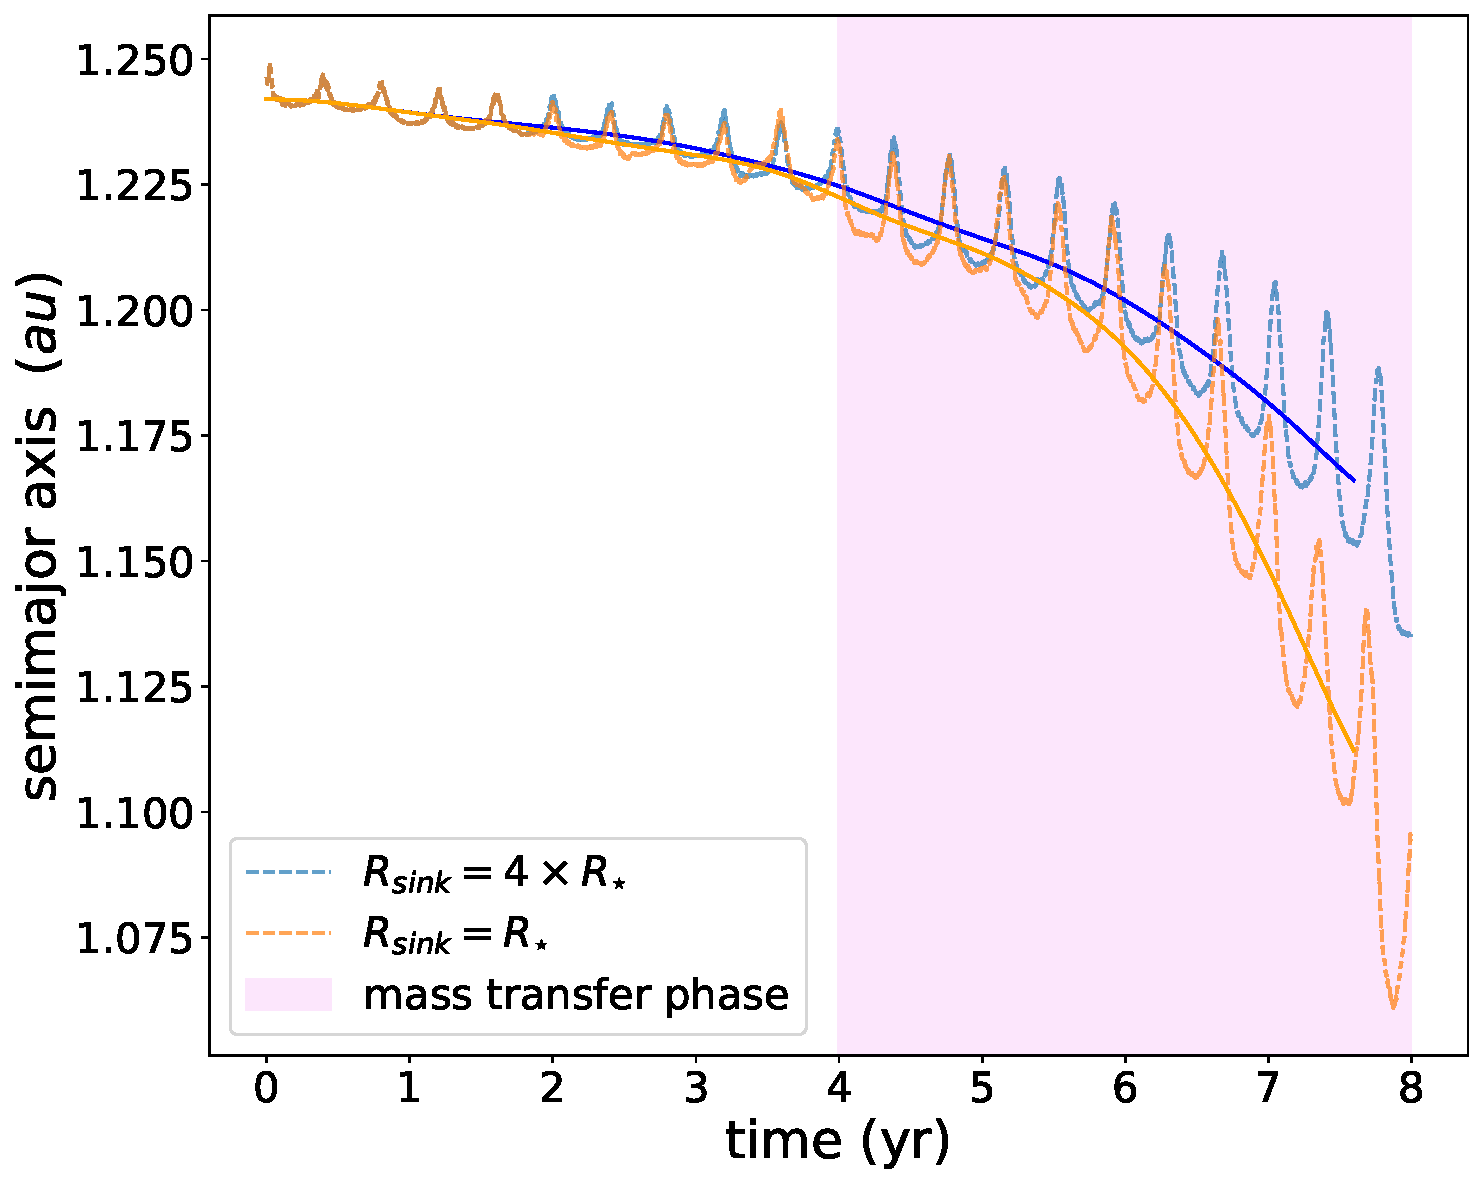
\includegraphics[width=0.9\textwidth]{Thesis/graphs/accretion_case/accretion_outer_semimajor_axis.pdf}
    \caption{Evolution of the semi-major axis of the outer orbit for the minimum and maximum accretion case. The simulated data is shown in dashed lines. The continues lines are smooth representations of the simulated data in their respective colors. The last three orbits are not included in the smoothed version, because the lack of data above $8$ yr will erroneously flatten the slopes.}
    \label{fig:accretion_outer_semimajor_axis}
\end{figure}
\begin{figure}[H]
    \centering
    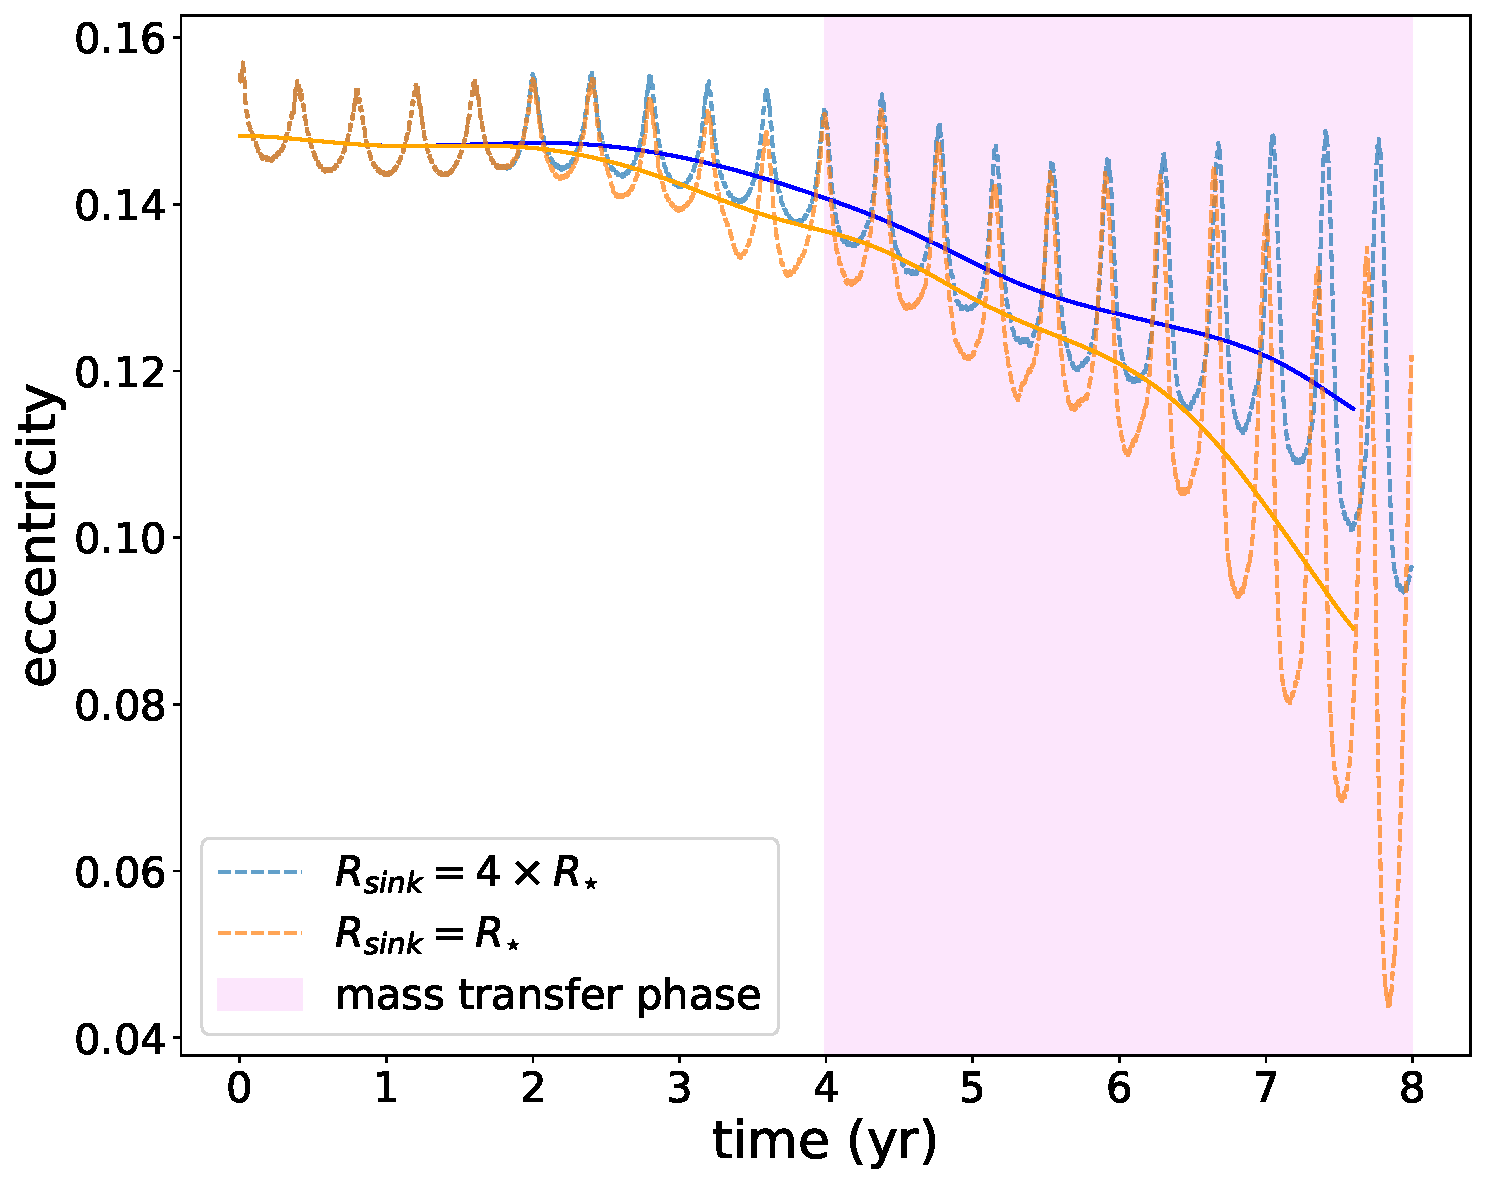
\includegraphics[width=0.76\textwidth]{Thesis/graphs/accretion_case/accretion_outer_ecc.pdf}
    \caption{Evolution of the eccentricity of the outer orbit for the minimum and maximum accretion case. The simulated data is shown in dashed lines. The continues lines are smooth representations of the simulated data in their respective colors. The last three orbits are not included in the smoothed version, because the lack of data above $8$ yr will erroneously flatten the slopes.}
    \label{fig:accretion_outer_ecc}
\end{figure}
\begin{comment}
\begin{figure}[H]
    \centering
    \begin{subfigure}{.5\textwidth}
    \centering
    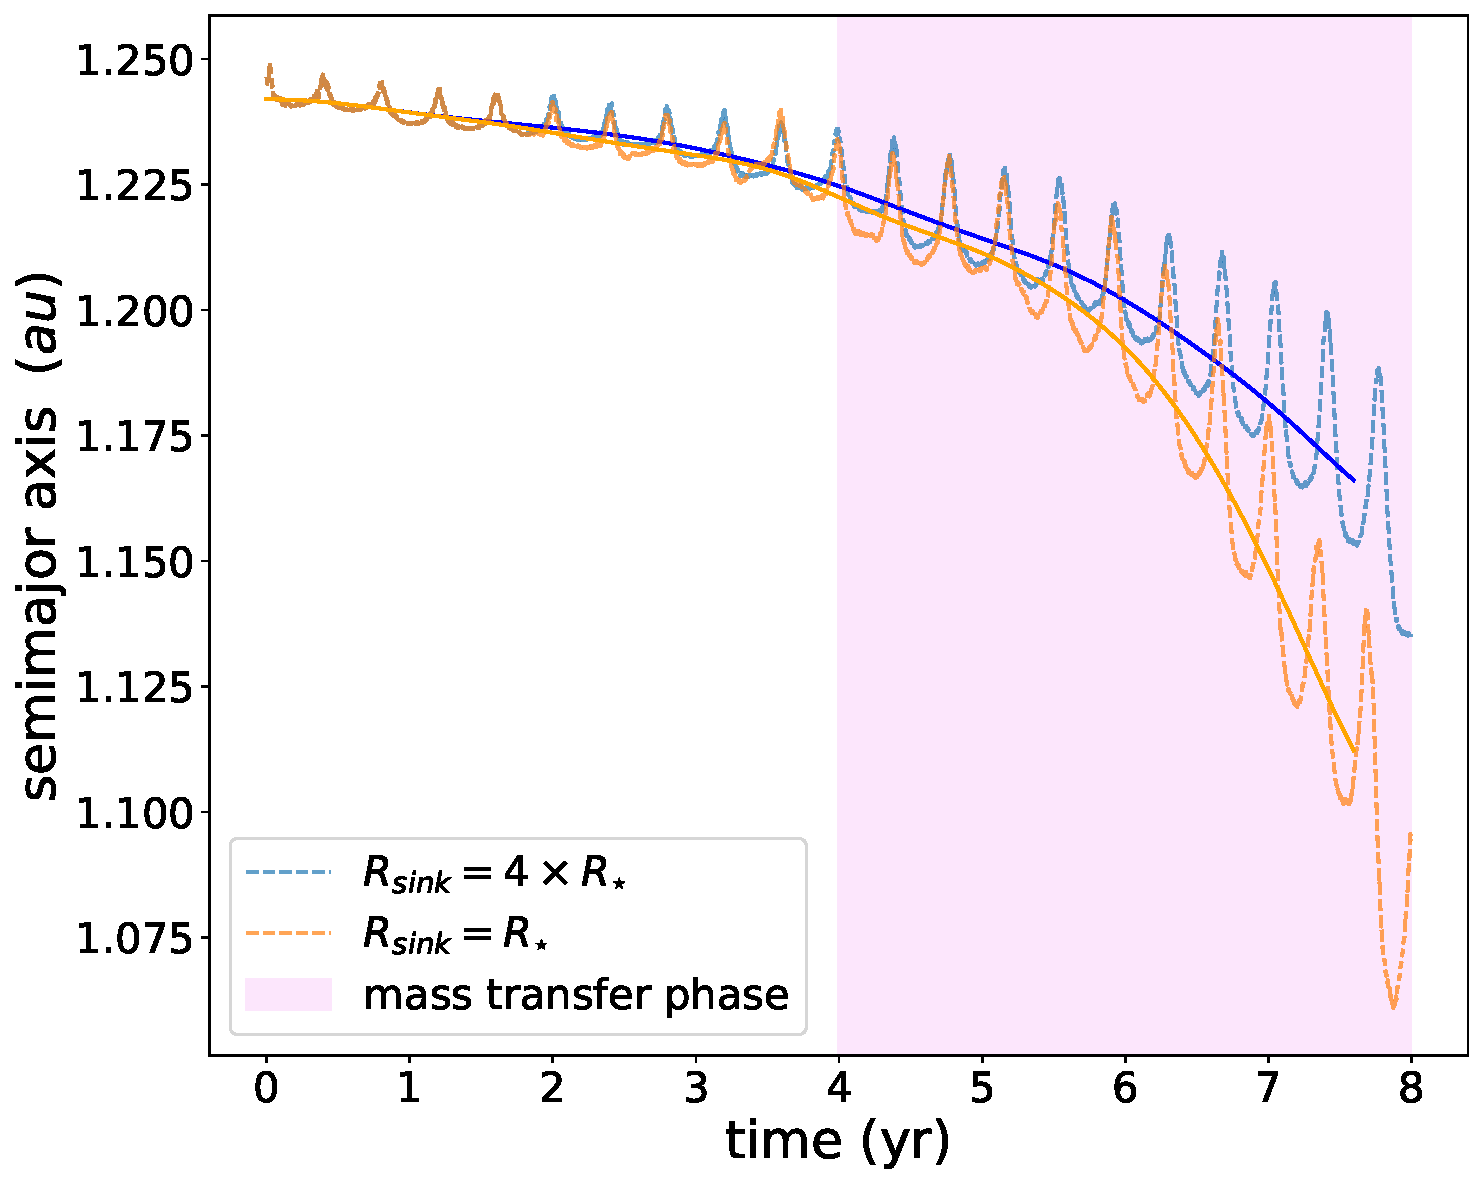
\includegraphics[width=0.9\textwidth]{Thesis/graphs/accretion_case/accretion_outer_semimajor_axis.pdf}
    \end{subfigure}%
    \begin{subfigure}{.5\textwidth}
    \centering
    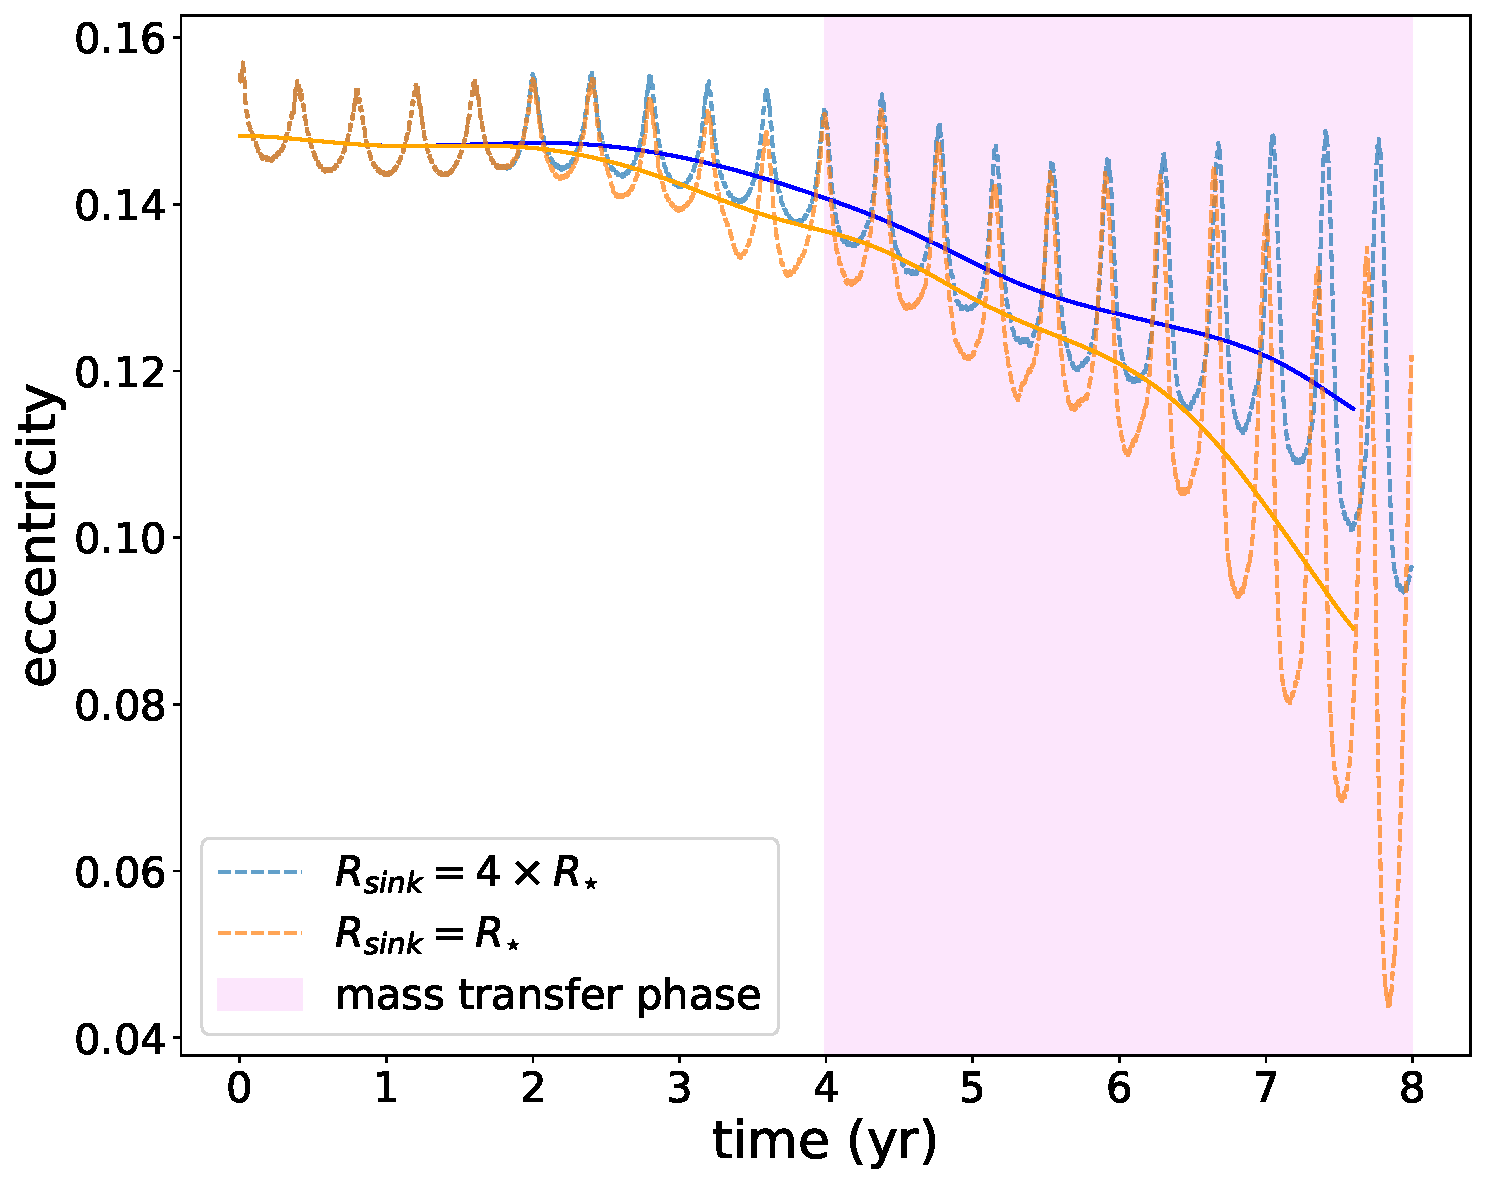
\includegraphics[width=0.9\textwidth]{Thesis/graphs/accretion_case/accretion_outer_ecc.pdf}
    \end{subfigure}
    \caption{ Evolution of the semi-major axis (left) and eccentricity (right) of the outer orbit}
    \label{fig:acc_outer_orbit}
\end{figure}
\end{comment}
\begin{figure}[!htb]
    \centering
    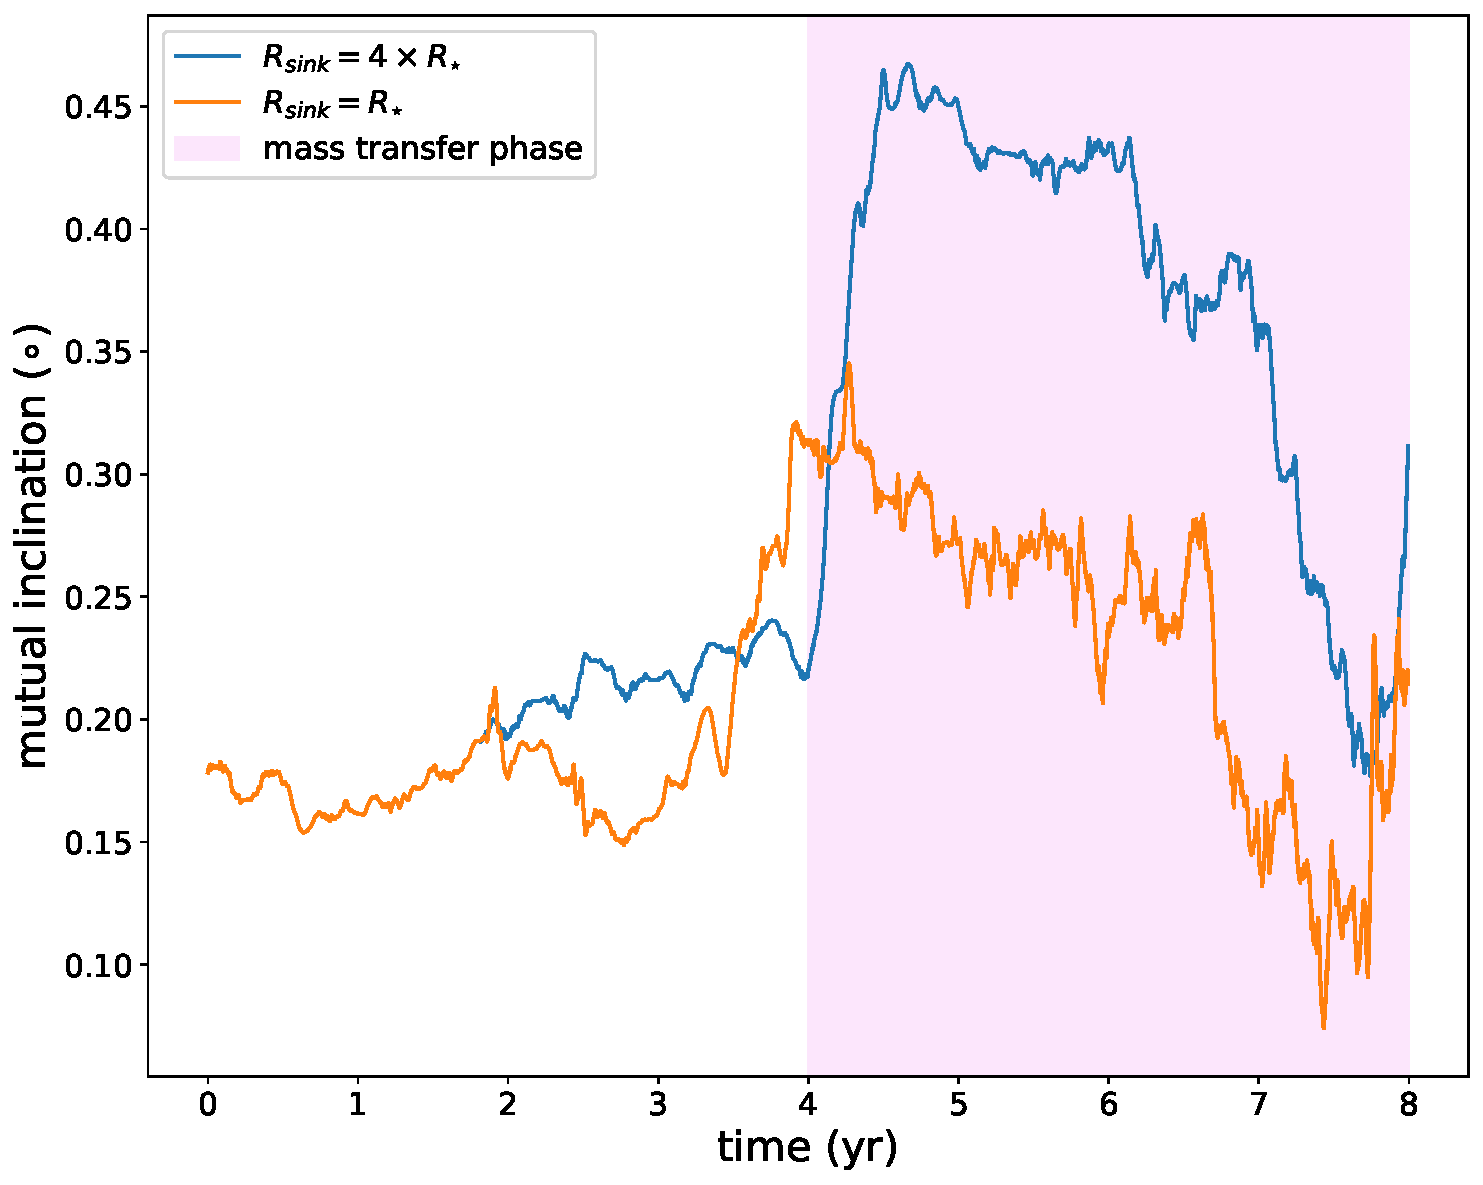
\includegraphics[width=0.76\textwidth]{Thesis/graphs/accretion_case/accretion_inc.pdf}
    \caption{Inclination of the outer orbit relative to the inner orbit.}
    \label{fig:accretion_inc}
\end{figure}
In \cref{fig:accretion_tertiary_mass}, I present the evolution of the tertiary's mass. The tertiary losses mass much faster in the minimum accretion case. The star's Roche lobe is proportional to its distance from the inner binary's center of mass; see \cref{eq:roche_lobe}, hence as the outer orbit decays faster, see \cref{fig:accretion_outer_semimajor_axis}, the tertiary's Roche lobe shrinks quicker. As a result, more and more gas overflows the Roche lobe and escapes towards the inner binary. To emphasize the difference in the mass evolution, I use central differentiation and provide mean mass loss rates for the simulated period, see \cref{fig:accretion_tertiary_mass}. The mass loss rates, should be taken with a grain of salt. Because the choice of $R_{\star} = 1.1 \times R_L$ significantly overestimates them, they should be treated qualitatively. Despite that, it can not be ignored that the simulated values are in very good agreement with analytical ones calculated using \cref{eq:mass_loss_rate_anal}.
\begin{figure}[H]
    \centering
    \begin{subfigure}{.5\textwidth}
    \centering
    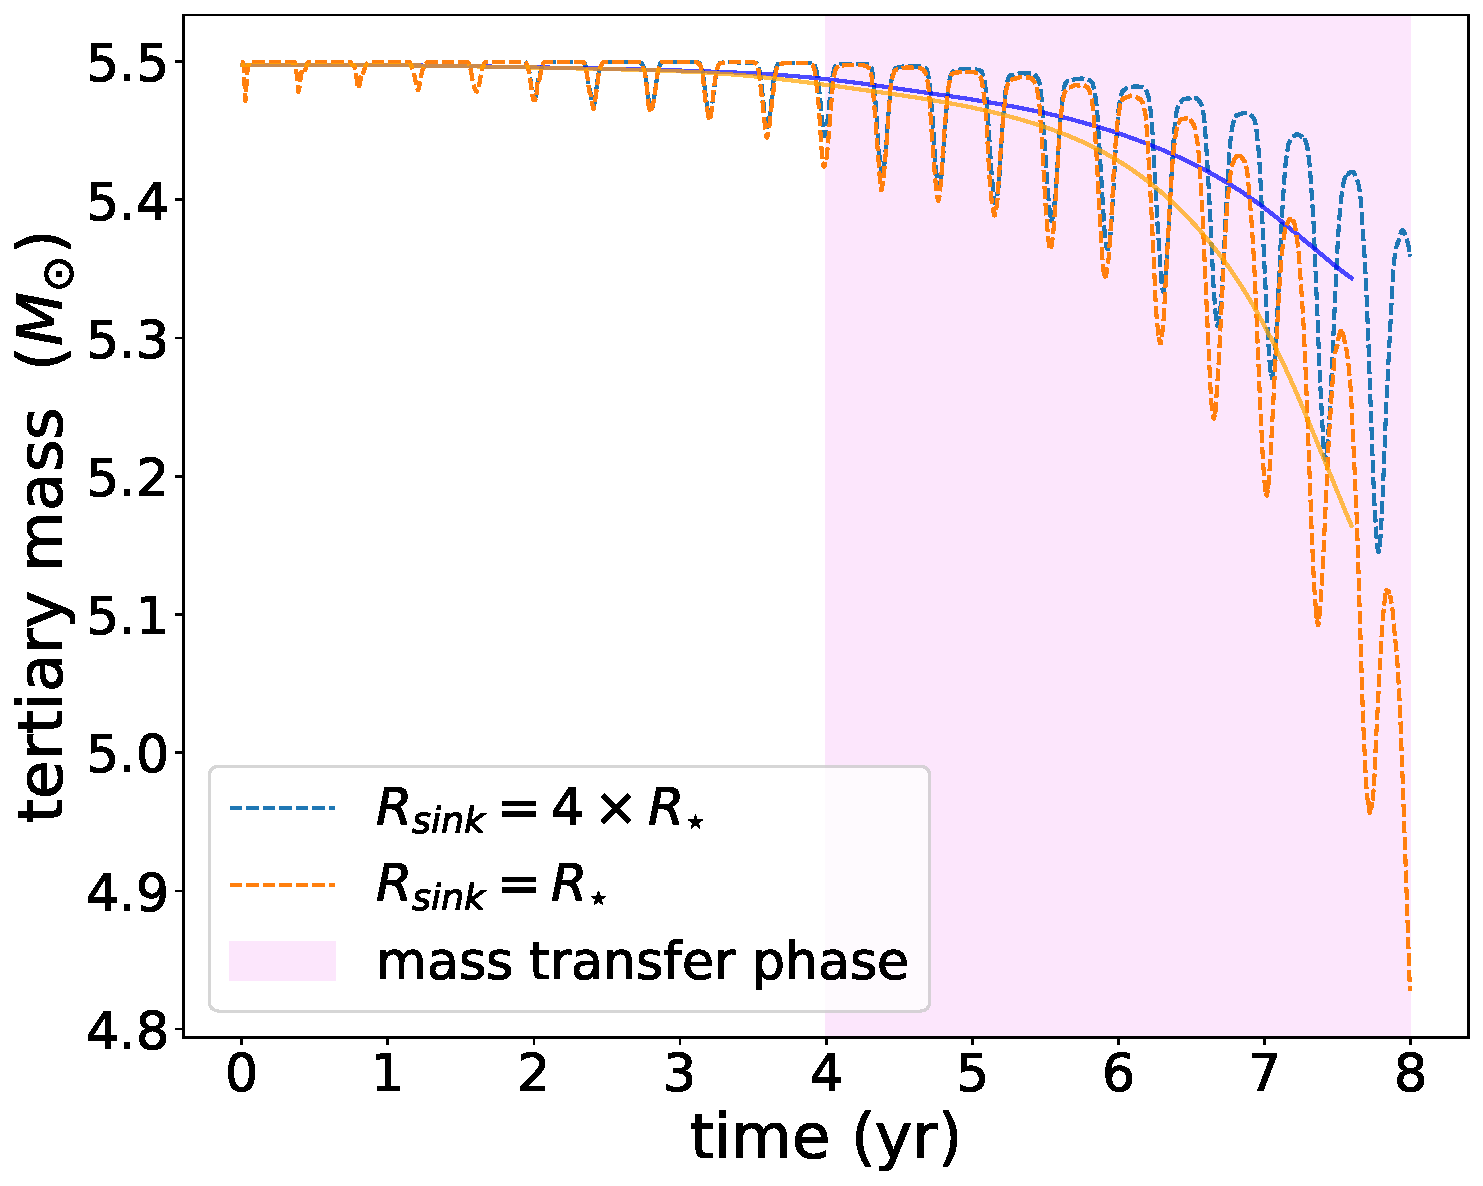
\includegraphics[width=0.9\textwidth]{Thesis/graphs/accretion_case/accretion_mass_loss.pdf}
    \end{subfigure}%
    \begin{subfigure}{.5\textwidth}
    \centering
    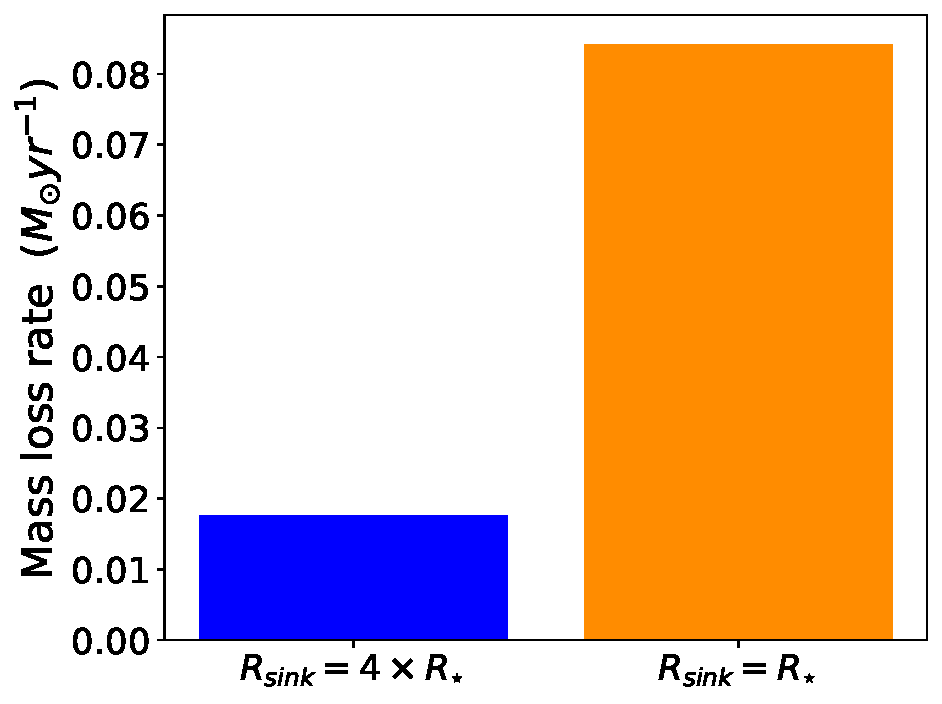
\includegraphics[width=0.9\textwidth]{Thesis/graphs/accretion_case/accretion_giant_mass_loss_rate.pdf}
    \end{subfigure}
    \caption{ The evolution of the tertiary's mass (left) for the minimum and maximum accretion case. The simulated data is shown in dashed lines. The continues lines are smooth representations of the simulated data in their respective colors. The last three orbits are not included in the smoothed version, because the lack of data above $8$ yr will erroneously flatten the slopes. The mean mass loss rates computed using central differentiation on the simulated data (right).}
    \label{fig:accretion_tertiary_mass}
\end{figure}


\subsection{Inner orbit}

In \cref{fig:accretion_inner_semimajor_axis} and \cref{fig:accretion_inner_ecc}, I present the evolution of the semi-major axis and eccentricity of the inner orbit, 
respectively. The initial inner and outer orbital angular momentum vectors are parallel and the inner orbit widens in both models as discussed in \cref{sec:resolution}. However, in the minimum accretion case, the orbit widens faster, see \cref{fig:accretion_inner_semimajor_axis}.
\begin{figure}[H]
    \centering
    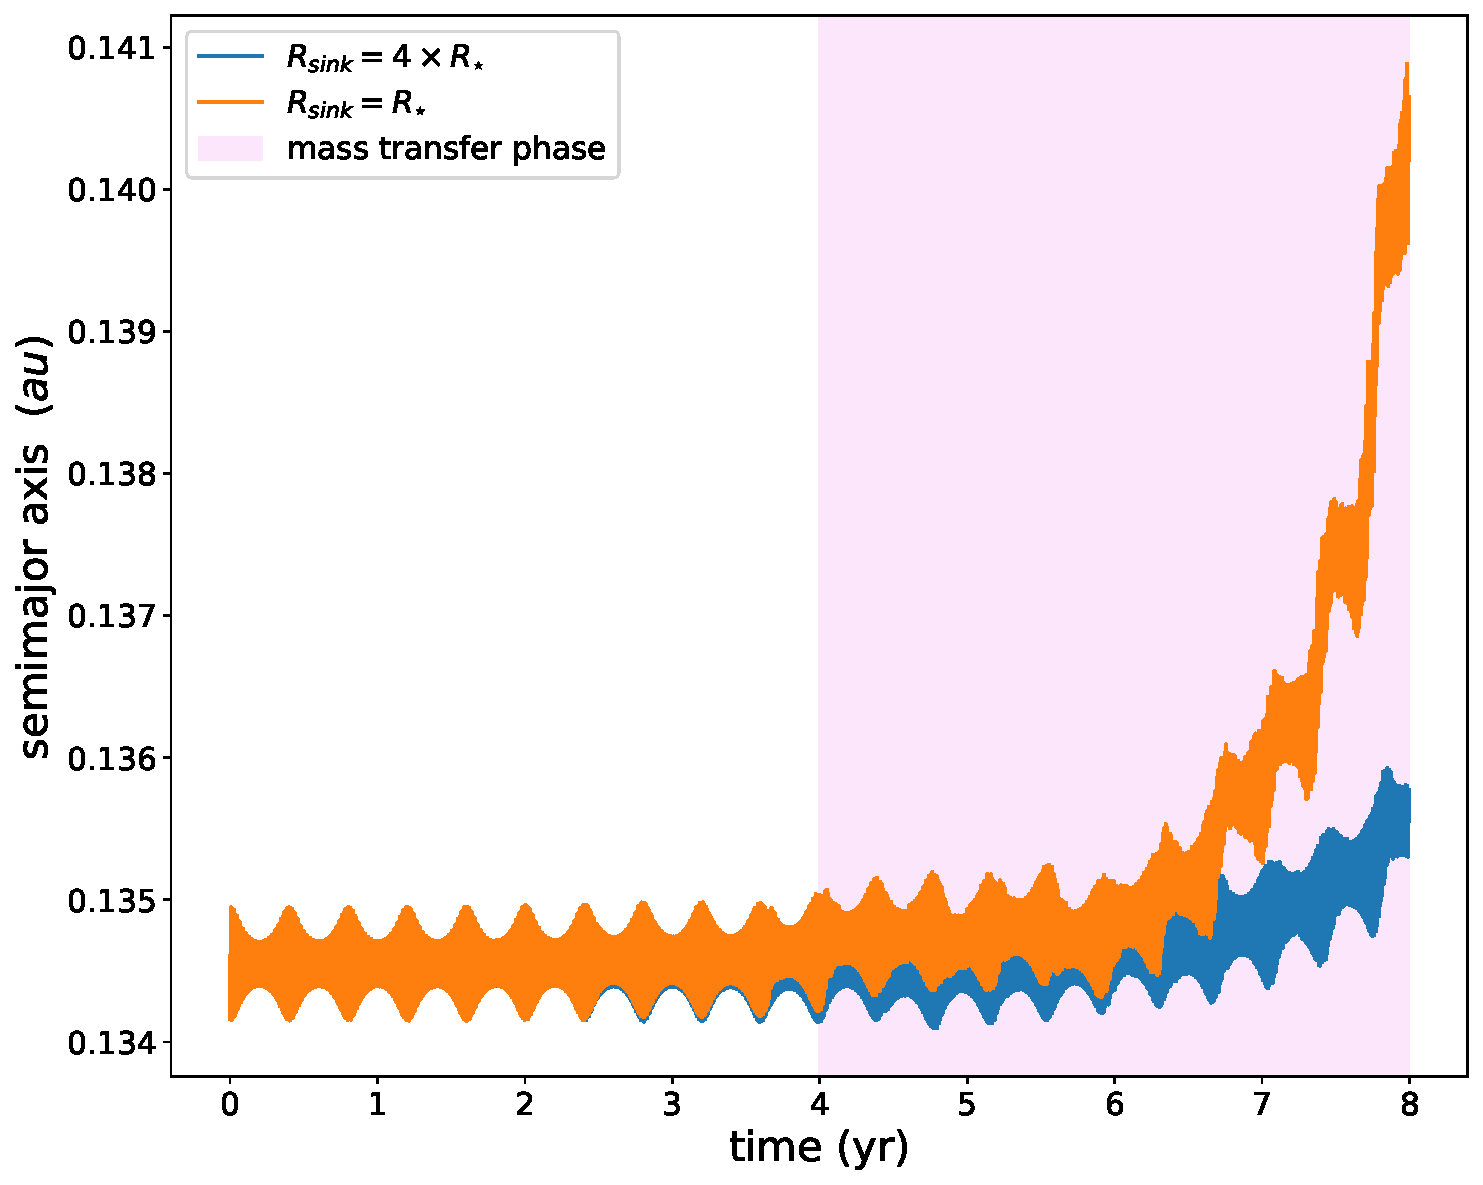
\includegraphics[width=0.9\textwidth]{Thesis/graphs/accretion_case/accretion_inner_semimajor_axis.pdf}
    \caption{Evolution of the semi-major axis of the inner orbit for the minimum and maximum accretion case.}
    \label{fig:accretion_inner_semimajor_axis}
\end{figure} 
The tertiary mass loss rate in the minimal accretion model is substantially larger than in the maximal accretion one, as seen \cref{fig:accretion_tertiary_mass}. Due to the underestimation of the effect of gas drag, the models are influenced by the gravitational interaction between the binary components and the incoming mass stream. As more mass approaches the binary components, in the minimum accretion case, it can also approach them closer before it is accreted, increasing the magnitude of the gravitational interactions. In conclusion, it is not possible to confidently draw conclusions about the impact of accretion on the inner orbit's semi-major axis given the current resolution. Finally, as expected, the effect of accretion on the eccentricity of the inner orbit is negligible. The orbit remains circular in both cases.
\begin{figure}[H]
    \centering
    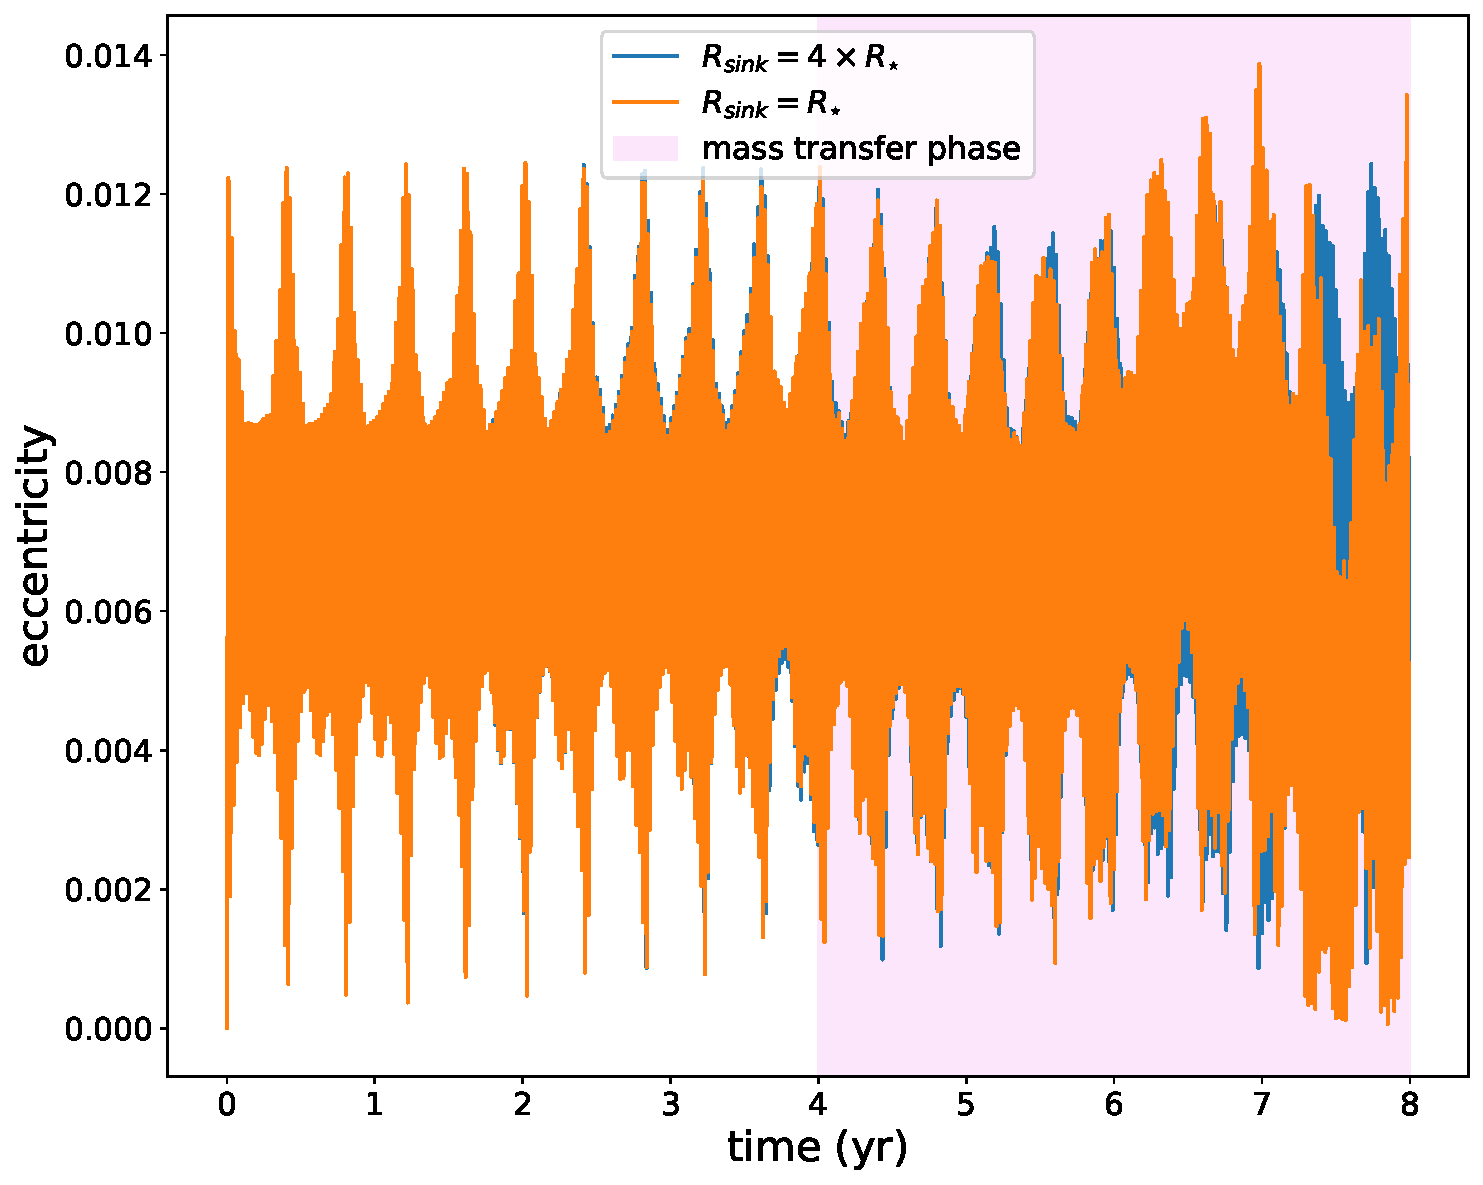
\includegraphics[width=0.9\textwidth]{Thesis/graphs/accretion_case/accretion_inner_ecc.pdf}
    \caption{Evolution of the eccentricity of the inner orbit for the minimum and maximum accretion case.}
    \label{fig:accretion_inner_ecc}
\end{figure}

\subsection{Analytical estimations}

During RLOF, matter from the outer donor star is either accreted onto the inner binary stars, forms a disc around them, or is expelled from the triple system entirely. The orbits will change depending on what happens to the mass. This may be expressed in terms of the amount of angular momentum carried by the mass as it exits the donor star. On the one hand, the fraction of the accreted mass, $\beta$, and the amount of angular momentum that is carried away by the escaping mass are highly uncertain, already in binary evolution studies. On the other hand, there are practically no theoretical predictions of the aforementioned quantities for mass transfer in hierarchical triples. More specifically, for the case of RLOF by an outer star towards the inner binary. 

In \cref{fig:accretion_eff_binary} I present an estimation of the accretion efficiency, $\beta$, for the maximum and minimum accretion models.
\begin{figure}[!htb]
    \centering
    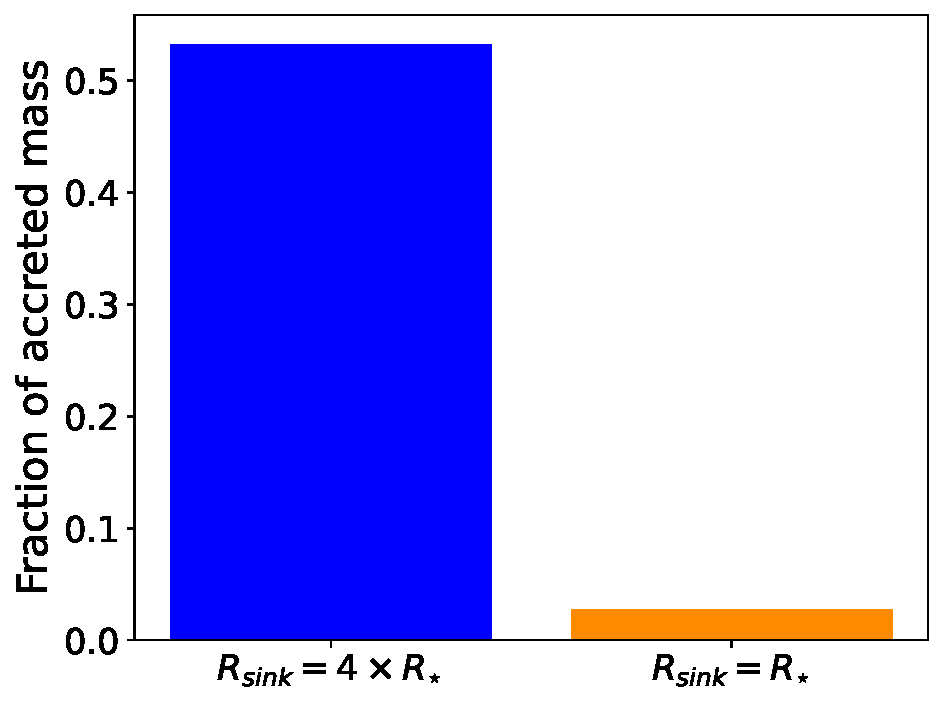
\includegraphics[width=0.9\textwidth]{Thesis/graphs/accretion_case/accretion_binary_acc_efficiency.pdf}
    \caption{Fraction of the accreted mass by the inner binary stars for the maximum and minim accretion cases.}
    \label{fig:accretion_eff_binary}
\end{figure}
In contrast to the concepts introduced in \cref{sub:orbit_evol_mass_loss}, $\beta$ here, corresponds to the fraction of mass that is accreted by the inner binary. Nonetheless, I find $\beta = 0.53$ and $\beta = 0.03$ for the maximum and minimum accretion case, respectively. 

The absolute values presented, however, should be taken with a grain of salt. Higher resolution simulations are needed to examine the evolution of the inner semi-major axis, which may alter the details of the accretion process. Furthermore, the short period simulated here, can not capture additional parameters, which affect the fraction of accreted mass, $\beta$, at later stages such as the response of the donor and accreting stars. For a detailed review I direct the reader to Onno Pols `Binary Stars`. Despite the aforementioned uncertainties, the above outcome hints an intriguing statement. Even though, the set up of the maximum accretion model intents to approach a conservative mass transfer scenario, the later is highly non-conservative. In comparison, theoretical studies of conservative mass transfer in binaries assume values of $\beta \geq 0.9$,

On the one hand, the low resolution of the simulation and thus the underestimation of the gas drag does not allow for a direct comparison between analytical models and the evolution of the inner orbit's semi-major axis. On the other hand, the gas drag on the inner binary is mostly irrelevant for the evolution of the semi-major axis of the outer orbit, thus the amount of the lost angular momentum can be parameterized using analytical models.

In order to get an estimation about how much angular momentum is lost from the system, I compare the evolution of the semi-major axis of the outer orbit with the analytical model for non-conservative mass transfer based on mass redistribution, see \cref{eq:semimajor_axis_no_cons}. The model assumes conservation of angular momentum despite the non-conservative case, similar to binaries as discussed by \cite{portegies1995formation}. Furthermore, it is assumed that the binary components are orbiting on the same plane, thus I compare the analytical model only with the models where $i_{mut}=0^{\circ}$, see \cref{tab:simulations_settings}.

Due to the fact that one component of the outer orbit is a binary system, the $M_a$ corresponds to its combined mass and $\eta$ is the specific angular momentum of the mass leaving the system as a proportion of the inner binary system's specific angular momentum. 
\begin{figure}[!htb]
    \centering
    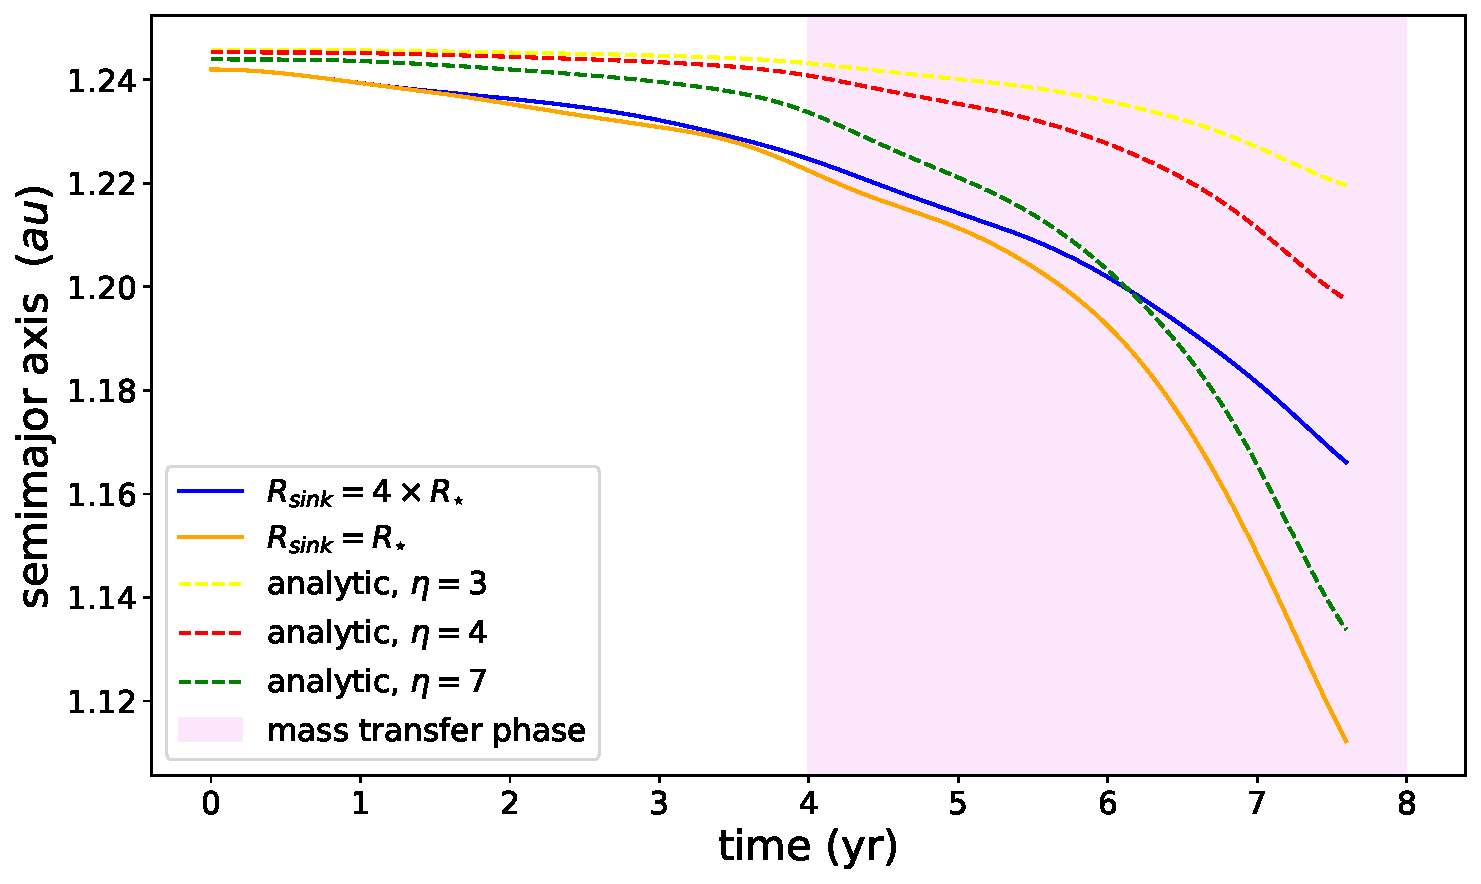
\includegraphics[width=0.85\textwidth]{Thesis/graphs/analytical_model.pdf}
    \caption{Evolution of the semi-major axis of the outer orbit for models number 1 and 4 listed in \cref{tab:simulations_settings}. The continues lines are representations of the simulated data, smoothed with a kernel with width $= 3 \times P_{out}$. The dashed lines correspond to analytical models in yellow, red, green and black, respectively.  The last three orbits are not included in the smoothed version, because the lack of data above $8$ yr will erroneously flatten the slopes.}
    \label{fig:comparison_analytical_model_max}
\end{figure}
In \cref{fig:comparison_analytical_model_max}, I present smoothed versions of the simulated data in blue and orange for the maximum and minimum accretion case, respectively. In the minimum accretion model, more than $99\%$ of the transferred mass is lost, this seems extremely high, even for a highly non-conservative mass transfer. Hence, I overplot four models, based on the maximum accretion model using \cref{eq:semi-major_axis}, for $\eta = 3,4,7,10$. Higher value of $\eta$ indicate that a higher amount of angular momentum is carried away by the ejected mass. During the mass transfer phase a model with $\eta \approx 4$ matches the slope of the orbital evolution for the maximum accretion case, while a model with $\eta \approx 7$ matches the minimum accretion case's orbital evolution slope. The graph indicates that in the maximum accretion case, given the same amount of ejected mass, the latter should carry significantly more angular momentum in order to match the minimum accretion case ($\eta = 7$). 

In conclusion, it is evident that the efficiency of the accretion process is vital for the timescale of the outer orbit's decay and consequently for the triple system's evolution. On the one hand, low values of $\beta$ are connected with a more unstable system. As angular momentum is lost rapidly, the fraction of the inner and outer orbit changes in ashorter timescale. Hence, the system enters the unstable regime quicker. Close encounters and collisions are expected to be enhanced, which tend to dissolve systems to lower orders \citep{van2007formation}. On the other hand, high values of $\beta$ are related to a somehow more stable system as less amount of angular momentum is lost, at least during the early phase of the mass transfer. The latter is expected to be somehow more stable and to extend during longer timescales.

Keep in mind that this analysis is focused solely on the response of the outer orbit to angular momentum loss under the assumption of the same amount of ejected mass. The overall stability of the mass transfer process is more strongly related to the donor mass loss rate, which strongly dependents on its envelope. For convective envelopes, the mass transfer is expected to become progressively more unstable, while radiative envelopes ensure that the mass transfer will be maximally conservative. A detailed analysis of the aforementioned topic is provided in Onno Pols `Binary Stars` and a more extensive discussion is taking place in \cref{sec:discussion}.


